\documentclass[polish, 11pt, a4paper]{article}

\usepackage{polski}
\usepackage[utf8]{inputenc}
\usepackage[autostyle]{csquotes}
\DeclareQuoteAlias{dutch}{polish}
\usepackage[T1]{fontenc}
\usepackage{geometry}
\geometry{
	a4paper,
	total={170mm,257mm},
	left=25mm,
	right=25mm,
	top=20mm,
}

\usepackage{babel}
\usepackage{microtype}
\usepackage{lmodern}
\usepackage{multirow}
\usepackage{array}
\newcolumntype{?}[1]{!{\vrule width #1}}
\usepackage{siunitx}
\usepackage{amsmath}
\usepackage{caption}
\usepackage{graphicx}
\usepackage{graphics}
\usepackage{float}
\usepackage{enumitem}
\usepackage{ragged2e}
\usepackage{parskip}
\RaggedRightParindent=24pt
\usepackage{indentfirst}
\usepackage[figurename=Wykres]{caption}

\begin{document}
	\begin{titlepage}
	\centering
	\Huge Laboratorium Podstaw Fizyki\\
	\vspace{1cm}
	\huge Ćwiczenie 48 \enquote{Wyznaczenie stałej Plancka na podstawie charakterystyki diody elektroluminescencyjnej}\\
	\vspace{1cm}
	\raggedright
	\huge Prowadzący: mgr Karolina Paradowska\\
	\vspace{.5cm}
	\begin{table}[h]
		\centering
		\resizebox{\columnwidth}{!}{%
		\begin{tabular}{|r|l|}\hline
			Imię i Nazwisko	&Marcin Kotas\\\hline
			Nr indeksu		&235098\\\hline
			Wydział			&Elektroniki\\\hline
			Termin zajęć	&28.11.2017, godz. 9.15\\\hline
			Numer grupy ćwiczeniowej&5\\\hline
			Data oddania sprawozdania&7.12.2017\\\hline
		\end{tabular}%
		}
	\end{table}
	\end{titlepage}
	\section{Wstęp teoretyczny}
		\RaggedRight
		Celem ćwiczenia było obliczenie stałej Plancka na podstawie charakterystyki diody elektroluminescencyjnej w kierunku przewodzenia oraz długości fali promieniowania emitowanego przez diodę.
		Wartość stałej Plancka wyznacza się z następującego wzoru:
		\begin{equation}
			h=\frac{e}{c}\lambda U_B
		\end{equation}
		gdzie:
		\begin{description}[align=right,labelwidth=6cm]
			\item[\(h{[J\cdot s]}\)] stała Plancka
			\item[\(e=1,602\times 10^{-19}{[C]}\)] elementarny ładunek elektryczny
			\item[\(c=299 792 458 {[\frac{m}{s}]}\)] prędkość światła w próżni
			\item[\(\lambda{[m]}\)] długość fali promieniowania emitowanego przez diodę
			\item[\(U_B{[V]}\)] bariera potencjału
		\end{description} 
		
	\section{Wyniki pomiarów}
		
	\subsection{Wykonanie pomiarów}
		Pomiary zostały wykonane dla 3 diod - żółtej, niebieskiej oraz zielonej.
		Dla każdej diody zmierzona została charakterystyka prądowo-napięciowa: napięcie zmieniane było co \(0,25 V\) aż do uzyskania niezerowej wartości natężenia.
		Od tego momentu wartości napięcia i natężenia zapisywane były co \(1mA\).
		Wyniki tych pomiarów przedstawione są w Tabelach 1-3.
		Na koniec zmierzona została raz długość fali światła emitowanego przez każdą diodę przy pomocy monochromatora.
		Zmierzone długości fal zapisane są w Tabeli 4.
	\subsection{Obliczenia}
	
	\subsubsection{Opracowanie wyników}
		Najpierw wykonane zostały wykresy charakterystyki I-V dla każdej diody - Wykresy 1-3.
		Następnie dopasowane zostały linie trendu dla wysokich prądów (\(>10mA\) dla diod żółtej i zielonej, \(>6mA\) dla diody niebieskiej).
		Miejse przecięcia linii trendu z osią poziomą wyznacza barierę potencjału \(U_B\). Dla diody żółtej:
		\begin{align*}
			A	&= 310,8082908 \approx 311\\			
			u(A)&=	10,20203602 \approx 11\\
			B	&=	-602,4185515 \approx -602\\
			u(B)&= 20,41717286 \approx 21\\			
			U_B	&=	\frac{-B}{A} = \frac{602}{311} = 1,938231924 \approx 1,938 [V]			
		\end{align*}
		Niepewność wyznaczonego potencjału została wyznacza ze wzoru:
		\begin{align*}
			u(V_B)	&= \sqrt{\left(-\frac{u(B)}{A}\right)^2+\left(-\frac{u(A)\cdot B}{A^2}\right)^2}
					 = \sqrt{\left(-\frac{21}{311}\right)^2+\left(-\frac{11\cdot (-602)}{311^2}\right)^2}\\
					& = 0,091448746	\approx 0,092 [V]
		\end{align*}	

		Błąd pomiarów napięcia oraz natężenia został wyliczony według wzorów podanych w specyfikacji miernika. Dla pomiaru nr.15 diody żółtej:
		\begin{align*}
			\Delta V&=\pm(0,9\%rdg+2dgt) = 0,009\cdot 1,936	+ 2\cdot 0,001 = 0,019424 [V]\\
			\Delta I&=\pm(1.4\%rdg+3dgt) = 0,014\cdot 6,01 + 3\cdot 0,01 = 0,11414 [mA]
		\end{align*}
		Niepewność tych pomiarów jest niepewnością typu B. Przyrząd pomiarowy był elektroniczny, więc niepewność zaokrąglona jest do rozdzielczości wyświetlanego wyniku:
		\begin{align*}
			u(V) &= \frac{\Delta V}{\sqrt{3}} = \frac{0,019424}{\sqrt{3}} = 0,011214452	\approx 0,012 [V]\\[10pt]
			u(I) &= \frac{\Delta I}{\sqrt{3}} = \frac{0,11414}{\sqrt{3}} = 0,06589876 \approx 0,07 [mA]
		\end{align*}

		Zmierzona długość światła wyniosła \(\lambda = 585 nm\) dla diody żółtej. Dokładność pomiaru przy pomocy monochromatora wynosi \(\Delta \lambda = 5 nm\).
		Jest to niepewność typu B, więc
		\begin{displaymath}
			u(\lambda) = \frac{\Delta \lambda}{\sqrt{3}} = \frac{5}{\sqrt{3}} = 2,886751346	\approx 2,9 [nm]
		\end{displaymath}

	\subsubsection{Wyznaczenie stałej Plancka}
		Na podstawie tych pomiarów wyznaczona została stała Plancka wg. wzoru (1). Dla diody żółtej:
		\begin{align*}
			h	&=	\frac{e}{c}\lambda U_B	=	\frac{1,602\cdot 10^{-19}}{299792458}\cdot 585\cdot 10^{-9}\cdot 1,938	=	6,05903\cdot 10^{-34}	\approx 6,06\cdot 10^{-34} [J\cdot s]			
		\end{align*}
		Niepewnosć tego pomiaru jest niepewnością złożoną:
		\begin{align*}
			u_c(h)	&=\sqrt{\left(\frac{\partial h}{\partial \lambda}\right)^2\cdot u^2(\lambda)+\left(\frac{\partial h}{\partial U_B}\right)^2\cdot u^2(U_B)}
					=\sqrt{\left(\frac{e}{c}\cdot U_B\right)^2\cdot u^2(\lambda) + \left(\frac{e}{c}\cdot \lambda\right)^2\cdot u^2(U_B)}\\[6pt]
					&=\sqrt{
						\begin{aligned}
						&\left(\frac{1,602\cdot 10^{-19}}{299792458}\cdot 1,938\right)^2\cdot (2,9\cdot 10^{-9})^2\\
						&+\left(\frac{1,602\cdot 10^{-19}}{299792458}\cdot 585\cdot 10^{-9}\right)^2\cdot 0,092^2
						\end{aligned}
					} = 0,287448\cdot 10^{-34}	\approx 0,29\cdot 10^{-34} [J\cdot s]
		\end{align*}
		Średnia stała Plancka na podstawie 3 pomiarów przy wykorzystaniu różnych diod wynosi:
		\begin{align*}
			\bar{h} = \frac{1}{3}\sum_{i=1}^{3}h_i=\frac{1}{3}(6,06 + 7,32 + 5,79)=\frac{1}{3}\cdot 19,17 = 6,39\cdot 10^{-34} [J\cdot s]			
		\end{align*}
		Niepewność średniej stałej Plancka jest odchyleniem standardowym pomiarów:
		\begin{displaymath}
			u(\bar{h})=\sqrt{\frac{\sum_{i=1}^{3}(h_i-\bar{h})^2}{3-1}} = 0,818323\cdot 10^{-34}	\approx 0,82 \cdot 10^{-34} [J\cdot s]
		\end{displaymath}
	\newpage
	\subsection{Tabele i wykresy}
		
		\begin{table}[H]
			\begin{minipage}{.5\textwidth}
				\centering
				\caption{Wyniki pomiarów dla diody żółtej}
				\begin{tabular}{|r|S[table-format=1.3, output-decimal-marker = {,}]|S[table-format=1.3, output-decimal-marker = {,}]|S[table-format=1.2, output-decimal-marker = {,}]|S[table-format=1.2, output-decimal-marker = {,}]|}\hline
					&&&&\\[-1em]
					Lp	&	{\(U [V]\)}	&	{\(u(U) [V]\)}	&	{\(I [mA]\)}	&	{\(u(I) [mA]\)}	\\\hline
					1	&	0,000	&	0,002	&	0,00	&	0,02	\\\hline
					2	&	0,251	&	0,003	&	0,00	&	0,02	\\\hline
					3	&	0,514	&	0,004	&	0,00	&	0,02	\\\hline
					4	&	0,757	&	0,006	&	0,00	&	0,02	\\\hline
					5	&	1,006	&	0,007	&	0,00	&	0,02	\\\hline
					6	&	1,250	&	0,008	&	0,00	&	0,02	\\\hline
					7	&	1,502	&	0,009	&	0,00	&	0,02	\\\hline
					8	&	1,750	&	0,011	&	0,22	&	0,02	\\\hline
					9	&	1,830	&	0,011	&	1,00	&	0,03	\\\hline
					10	&	1,872	&	0,011	&	2,00	&	0,04	\\\hline
					11	&	1,897	&	0,012	&	3,03	&	0,05	\\\hline
					12	&	1,913	&	0,012	&	4,02	&	0,05	\\\hline
					13	&	1,926	&	0,012	&	5,03	&	0,06	\\\hline
					14	&	1,936	&	0,012	&	6,01	&	0,07	\\\hline
					15	&	1,945	&	0,012	&	7,00	&	0,08	\\\hline
					16	&	1,952	&	0,012	&	8,00	&	0,09	\\\hline
					17	&	1,960	&	0,012	&	9,18	&	0,10	\\\hline
					18	&	1,965	&	0,012	&	10,08	&	0,10	\\\hline
					19	&	1,971	&	0,012	&	11,06	&	0,11	\\\hline
					20	&	1,976	&	0,012	&	12,11	&	0,12	\\\hline
					21	&	1,981	&	0,012	&	13,11	&	0,13	\\\hline
					22	&	1,985	&	0,012	&	14,07	&	0,14	\\\hline
					23	&	1,989	&	0,012	&	15,06	&	0,14	\\\hline
					24	&	1,992	&	0,012	&	16,10	&	0,15	\\\hline
					25	&	1,995	&	0,012	&	17,00	&	0,16	\\\hline
					26	&	1,999	&	0,012	&	18,07	&	0,17	\\\hline
					27	&	2,002	&	0,012	&	19,09	&	0,18	\\\hline
					28	&	2,006	&	0,012	&	20,16	&	0,19	\\\hline
					29	&	2,008	&	0,012	&	21,03	&	0,19	\\\hline
					30	&	2,011	&	0,012	&	22,03	&	0,20	\\\hline
					31	&	2,014	&	0,012	&	23,06	&	0,21	\\\hline
					32	&	2,016	&	0,012	&	24,05	&	0,22	\\\hline
					33	&	2,018	&	0,012	&	25,04	&	0,22	\\\hline
					34	&	2,021	&	0,012	&	26,12	&	0,23	\\\hline
					35	&	2,023	&	0,012	&	27,12	&	0,24	\\\hline
					36	&	2,025	&	0,012	&	28,03	&	0,25	\\\hline
					37	&	2,027	&	0,012	&	29,03	&	0,26	\\\hline
				\end{tabular}
			\end{minipage}%
			\begin{minipage}{.5\textwidth}	
				\centering
				\caption{Wyniki pomiarów dla diody niebieskiej}
				\begin{tabular}{|r|S[table-format=1.3, output-decimal-marker = {,}]|S[table-format=1.3, output-decimal-marker = {,}]|S[table-format=1.2, output-decimal-marker = {,}]|S[table-format=1.2, output-decimal-marker = {,}]|}\hline
					&&&&\\[-1em]
					Lp	&	{\(U [V]\)}	&	{\(u(U) [V]\)}	&	{\(I [mA]\)}	&	{\(u(I) [mA]\)}	\\\hline
					1	&	0,258	&	0,003	&	0,00	&	0,02	\\\hline
					2	&	0,501	&	0,004	&	0,00	&	0,02	\\\hline
					3	&	0,726	&	0,005	&	0,00	&	0,02	\\\hline
					4	&	1,000	&	0,007	&	0,00	&	0,02	\\\hline
					5	&	1,253	&	0,008	&	0,00	&	0,02	\\\hline
					6	&	1,500	&	0,009	&	0,00	&	0,02	\\\hline
					7	&	1,750	&	0,011	&	0,00	&	0,02	\\\hline
					8	&	2,000	&	0,012	&	0,00	&	0,02	\\\hline
					9	&	2,250	&	0,013	&	0,00	&	0,02	\\\hline
					10	&	2,501	&	0,015	&	0,00	&	0,02	\\\hline
					11	&	2,600	&	0,015	&	0,04	&	0,02	\\\hline
					12	&	2,815	&	0,016	&	1,00	&	0,03	\\\hline
					13	&	2,880	&	0,017	&	2,00	&	0,04	\\\hline
					14	&	2,925	&	0,017	&	3,01	&	0,05	\\\hline
					15	&	2,960	&	0,017	&	4,00	&	0,05	\\\hline
					16	&	2,992	&	0,017	&	5,02	&	0,06	\\\hline
					17	&	3,018	&	0,017	&	6,00	&	0,07	\\\hline
					18	&	3,043	&	0,017	&	7,03	&	0,08	\\\hline
					19	&	3,066	&	0,018	&	8,04	&	0,09	\\\hline
					20	&	3,087	&	0,018	&	9,09	&	0,10	\\\hline
					21	&	3,105	&	0,018	&	10,00	&	0,10	\\\hline
					22	&	3,124	&	0,018	&	11,01	&	0,11	\\\hline
					23	&	3,142	&	0,018	&	12,00	&	0,12	\\\hline
					24	&	3,160	&	0,018	&	13,00	&	0,13	\\\hline
					25	&	3,177	&	0,018	&	14,03	&	0,14	\\\hline
					26	&	3,194	&	0,018	&	15,07	&	0,14	\\\hline
					27	&	3,208	&	0,018	&	16,02	&	0,15	\\\hline
					28	&	3,224	&	0,018	&	17,05	&	0,16	\\\hline
				\end{tabular}
			\end{minipage}
		\end{table}
	
		\begin{table}[H]
			\begin{minipage}{.5\textwidth}
				\centering
				\caption{Wyniki pomiarów dla diody zielonej}
				\begin{tabular}{|r|S[table-format=1.3, output-decimal-marker = {,}]|S[table-format=1.3, output-decimal-marker = {,}]|S[table-format=1.2, output-decimal-marker = {,}]|S[table-format=1.2, output-decimal-marker = {,}]|}\hline
					&&&&\\[-1em]
					Lp	&	{\(U [V]\)}	&	{\(u(U) [V]\)}	&	{\(I [mA]\)}	&	{\(u(I) [mA]\)}	\\\hline
					1	&	0,000	&	0,002	&	0,00	&	0,02	\\\hline
					2	&	0,250	&	0,003	&	0,00	&	0,02	\\\hline
					3	&	0,500	&	0,004	&	0,00	&	0,02	\\\hline
					4	&	0,750	&	0,006	&	0,00	&	0,02	\\\hline
					5	&	1,000	&	0,007	&	0,00	&	0,02	\\\hline
					6	&	1,250	&	0,008	&	0,00	&	0,02	\\\hline
					7	&	1,500	&	0,009	&	0,00	&	0,02	\\\hline
					8	&	1,750	&	0,011	&	0,16	&	0,02	\\\hline
					9	&	1,835	&	0,011	&	1,00	&	0,03	\\\hline
					10	&	1,873	&	0,011	&	2,00	&	0,04	\\\hline
					11	&	1,896	&	0,012	&	3,00	&	0,05	\\\hline
					12	&	1,913	&	0,012	&	4,04	&	0,05	\\\hline
					13	&	1,926	&	0,012	&	5,02	&	0,06	\\\hline
					14	&	1,937	&	0,012	&	6,04	&	0,07	\\\hline
					15	&	1,946	&	0,012	&	7,04	&	0,08	\\\hline
					16	&	1,954	&	0,012	&	8,03	&	0,09	\\\hline
					17	&	1,958	&	0,012	&	9,05	&	0,10	\\\hline
					18	&	1,961	&	0,012	&	10,05	&	0,10	\\\hline
					19	&	1,965	&	0,012	&	10,99	&	0,11	\\\hline
					20	&	1,970	&	0,012	&	12,02	&	0,12	\\\hline
					21	&	1,976	&	0,012	&	13,04	&	0,13	\\\hline
					22	&	1,979	&	0,012	&	14,01	&	0,14	\\\hline
					23	&	1,983	&	0,012	&	15,06	&	0,14	\\\hline
					24	&	1,985	&	0,012	&	16,03	&	0,15	\\\hline
					25	&	1,988	&	0,012	&	17,03	&	0,16	\\\hline
					26	&	1,991	&	0,012	&	18,14	&	0,17	\\\hline
					27	&	1,994	&	0,012	&	19,07	&	0,18	\\\hline
					28	&	1,996	&	0,012	&	20,00	&	0,18	\\\hline
					29	&	1,999	&	0,012	&	21,00	&	0,19	\\\hline
					30	&	2,002	&	0,012	&	22,05	&	0,20	\\\hline
					31	&	2,005	&	0,012	&	23,03	&	0,21	\\\hline
					32	&	2,008	&	0,012	&	24,01	&	0,22	\\\hline
					33	&	2,011	&	0,012	&	25,10	&	0,23	\\\hline
					34	&	2,014	&	0,012	&	26,00	&	0,23	\\\hline
					35	&	2,015	&	0,012	&	27,02	&	0,24	\\\hline
					36	&	2,018	&	0,012	&	28,02	&	0,25	\\\hline
					37	&	2,020	&	0,012	&	29,16	&	0,26	\\\hline
				\end{tabular}
			\end{minipage}%
			\begin{minipage}{.5\textwidth}	
				\centering
				\caption{Końcowe wyniki pomiarów}
				\renewcommand{\arraystretch}{1.2}
				\begin{tabular}{|c|rl|S[table-format=3.3, output-decimal-marker = {,}]|S[table-format=1.3, output-decimal-marker = {,}]|}\cline{4-5}
					\multicolumn{3}{c|}{ }	&	{\(x\)}	&	{\(u(x)\)}	\\\hline
					\parbox[t]{2mm}{\multirow{3}{*}{\rotatebox[origin=c]{90}{żółta}}}	&	\(\lambda\)	&	 \([nm]\)	&	585,0	&	2,9	\\\cline{2-5}
																						&	\(U_B\)	&	\([V]\)	&	1,938	&	0,092	\\\cline{2-5}
																						& 	\(h\)	&	\(\times 10^{-34} [J\cdot s]\)	&	6,06	&	0,21	\\\hline
					\parbox[t]{2mm}{\multirow{3}{*}{\rotatebox[origin=c]{90}{niebieska}}}	&	\(\lambda\)	&	 \([nm]\)	&	470,0	&	2,9	\\\cline{2-5}
																						&	\(U_B\)	&	\([V]\)	&	2,915	&	0,095	\\\cline{2-5}
																						& 	\(h\)	&	\(\times 10^{-34} [J\cdot s]\)	&	7,32	&	0,25	\\\hline
					\parbox[t]{2mm}{\multirow{3}{*}{\rotatebox[origin=c]{90}{zielona}}}	&	\(\lambda\)	&	 \([nm]\)	&	560,0	&	2,9	\\\cline{2-5}
																						&	\(U_B\)	&	\([V]\)	&	1,935	&	0,070	\\\cline{2-5}
																						& 	\(h\)	&	\(\times 10^{-34} [J\cdot s]\)	&	5,79	&	0,21	\\\hline
					\multicolumn{1}{c|}{ }												& 	\(\bar{h}\)	&	\(\times 10^{-34} [J\cdot s]\)	&	6,39	&	0,82 \\\cline{2-5}
																						
				\end{tabular}
				\renewcommand{\arraystretch}{1}
			\end{minipage}
		\end{table}
		
		\begin{figure}[H]
    		\centering
    		\caption{charakterystyka I-V dla diody żółtej}
    		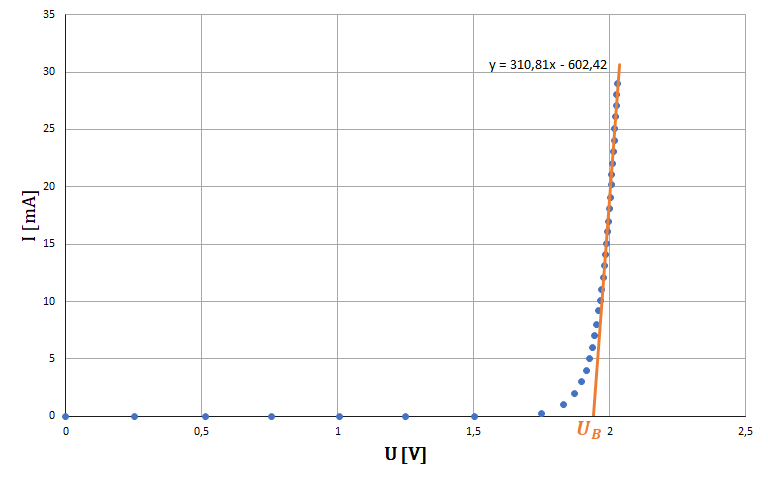
\includegraphics[width=\textwidth]{Fizyka48Wykres1}
		\end{figure}
		
		\begin{figure}[H]
    		\centering
    		\caption{charakterystyka I-V dla diody niebieskiej}
    		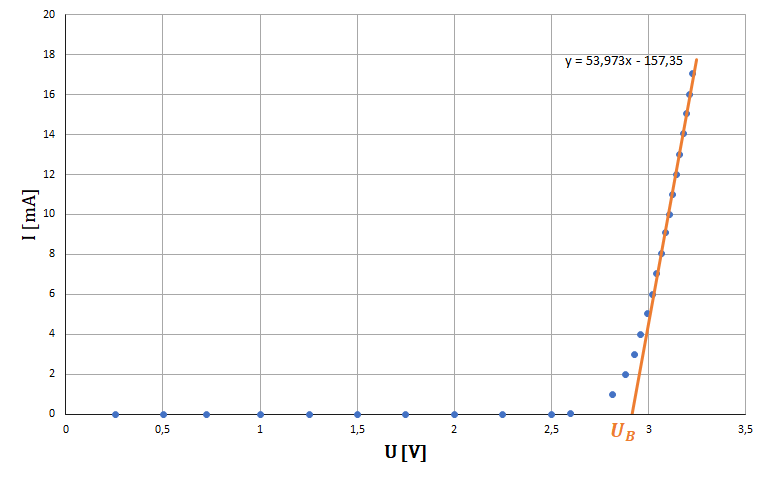
\includegraphics[width=\textwidth]{Fizyka48Wykres2}
		\end{figure}
		
		\begin{figure}[H]
    		\centering
    		\caption{charakterystyka I-V dla diody zielonej}
    		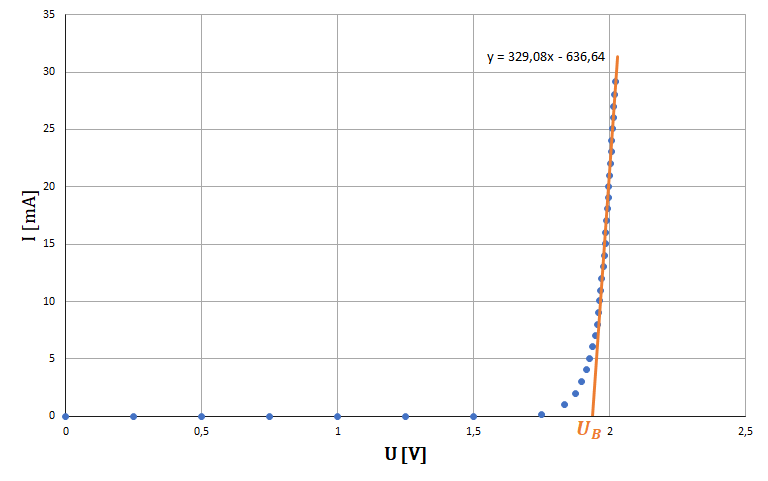
\includegraphics[width=\textwidth]{Fizyka48Wykres3}
		\end{figure}
		

	\section{Ostateczne wyniki}
		Ostateczne wyniki wraz z zaokrągleniami:
		\begin{description}[align=right,labelwidth=10cm]
			\item [Potencjał wbudowany diody żółtej:]{\((1,938\pm 0,0092)V\)}
			\item [Potencjał wbudowany diody niebieskiej:] {\((2,915\pm 0,095)V\)}
			\item [Potencjał wbudowany diody zielonej:] {\((1,935\pm 0,070)V\)}
			\item [Stała Plancka wyliczona na podstawie diody żółtej:] {\((6,06\pm 0,21)\times 10^{-34} J\cdot s\)}
			\item [Stała Plancka wyliczona na podstawie diody niebieskiej:] {\((7,32\pm 0,25)\times 10^{-34} J\cdot s\)}
			\item [Stała Plancka wyliczona na podstawie diody zielonej:] {\((5,79\pm 0,21)\times 10^{-34} J\cdot s\)}
			\item [Średnia stała Plancka:] {\((6,39\pm 0,82)\times 10^{-34} J\cdot s\)}
		\end{description}

	\section{Dyskusja i wnioski}
		Zbadana stała Plancka różni się dla poszczególnych diod. Wynika to głównie z jednorazowego, a więc niedokładnego pomiaru długości fali emitowanej przez diody.
		Średnia wartość, która wyniosła \((6,39\pm 0,82) \times 10^{-34}[J\cdot s]\) jest bliska wartości prawdziwej \(h\approx 6,626\times 10^{-34} [J\cdot s]\).
		Średnia wartość różni się od prawdziwej o zaledwie \(3,5 \%\), więc wyznaczona została z wysoką dokładnością.
		Najbliżej wartości prawdziwej znalazła się wartość wyznaczona przy pomocy diody żółtej.
\end{document}